\documentclass[a4paper,10pt]{article}

%A Few Useful Packages
\usepackage{marvosym}
\usepackage{fontspec} 					%for loading fonts
\usepackage{xunicode,xltxtra,url,parskip} 	%other packages for formatting
\RequirePackage{color,graphicx}
\usepackage[usenames,dvipsnames]{xcolor}
\usepackage[big]{layaureo} 				%better formatting of the A4 page
% an alternative to Layaureo can be ** \usepackage{fullpage} **
\usepackage{supertabular} 				%for Grades
\usepackage{titlesec}					%custom \section
\usepackage{graphicx}
%Setup hyperref package, and colours for links
\usepackage{hyperref}
\definecolor{linkcolour}{rgb}{0,0.2,0.6}
\hypersetup{colorlinks,breaklinks,urlcolor=linkcolour, linkcolor=linkcolour}
\usepackage{fontawesome}
\usepackage{setspace}

%FONTS
\defaultfontfeatures{Mapping=tex-text}
%\setmainfont[SmallCapsFont = Fontin SmallCaps]{Fontin}
%%% modified for Karol Kozioł for ShareLaTeX use
\setmainfont[
SmallCapsFont = Fontin-SmallCaps.otf,
BoldFont = Fontin-Bold.otf,
ItalicFont = Fontin-Italic.otf
]
{Fontin.otf}
%%%

%CV Sections inspired by: 
%http://stefano.italians.nl/archives/26
\titleformat{\section}{\Large\scshape\raggedright}{}{0em}{}[\titlerule]
\titlespacing{\section}{0pt}{3pt}{3pt}
%Tweak a bit the top margin
%\addtolength{\voffset}{-1.3cm}

%Italian hyphenation for the word: ''corporations''
\hyphenation{im-pre-se}

%-------------WATERMARK TEST [**not part of a CV**]---------------
\usepackage[absolute]{textpos}

\setlength{\TPHorizModule}{30mm}
\setlength{\TPVertModule}{\TPHorizModule}
\textblockorigin{2mm}{0.65\paperheight}
\setlength{\parindent}{0pt}

%--------------------BEGIN DOCUMENT----------------------
\begin{document}

%WATERMARK TEST [**not part of a CV**]---------------
%\font\wm=''Baskerville:color=787878'' at 8pt
%\font\wmweb=''Baskerville:color=FF1493'' at 8pt
%{\wm 
%	\begin{textblock}{1}(0,0)
%		\rotatebox{-90}{\parbox{500mm}{
%			Typeset by Alessandro Plasmati with \XeTeX\  \today\ for 
%			{\wmweb \href{http://www.aleplasmati.comuv.com}{aleplasmati.comuv.com}}
%		}
%	}
%	\end{textblock}
%}

\pagestyle{empty} % non-numbered pages

\font\fb=''[cmr10]'' %for use with \LaTeX command

%--------------------TITLE-------------

\par{

		{\Huge Karavaeva \textsc{Valeriia}
	}\hspace{4cm}
    % 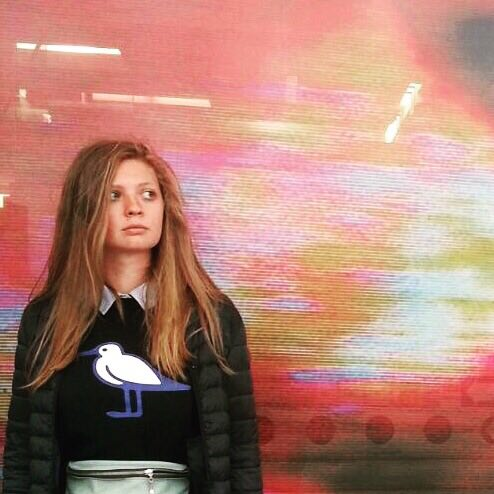
\includegraphics[scale=0.15]{1.jpg}
\par} 


%--------------------SECTIONS-----------------------------------
%Section: Personal Data
\section{Personal Data}

\begin{tabular}{rl}
    \textsc{Location:} & Saint Petersburg, Russia \\
    % \textsc{Date of Birth:} & 03 December 1992 \\
    %\textsc{Address:}   & CV Inn 19, 20301, Milano, Italy \\
    \textsc{Phone:}     & +79215780461\\
    \textsc{email:}     & \href{mailto:valerakaravai@gmail.com}{valerakaravai@gmail.com} \\
    \textsc{Other:}     &
\href{https://www.linkedin.com/in/valeriya-karavaeva/}{\ci{\faLinkedin}}
\href{https://github.com/ValeraKaravai}{\ci{\faGithub}}
\href{https://join.skype.com/invite/mHExCQKPdCGJ}{\ci{\faSkype}}
\end{tabular}

%Section: Work Experience at the top
\section{Work Experience}
\begin{tabular}{r|p{11cm}}
\textsc{May 2018} &\textbf{Project Spiking (Aly), Singapore} \\
  \textsc{CURRENT}&\emph{Data Scientist}\\
  {}&\href{https://spiking.io/}{https://spiking.io}\\
  {}&\begin{itemize}  
\item Application of machine learning problems in finance
\item Development of algorithm and pipeline for predicting anomalies (spike up/ spike down) of stock prices of campaigns using machine learning algorithms (using Tensorflow, online learning model)
\item Development of algorithm and pipeline for sentiment analysis for news processing
\item Crypto data. Development of algorithm for crypto address clustering
\end{itemize}
\textbf{Instruments}: Python, TensorFlow, Go, SQL, Airflow, Keras, Prometheus, Graphana  \\
& \\
\textsc{Sep 2016} & \textbf{PropellerAds, Russia} \\\textsc{Apr 2018}&\emph{Data Scientist}\\
{}&\begin{itemize}  
\item Development and implementation of advertising rotation algorithms
\item Introduction of algorithms for searching anomalies of company's business metrics
\item Development of an algorithm for searching for bot traffic
\item Development of a cold start method for testing advertising campaigns
\end{itemize}
\textbf{Instruments}: Python, R, TensorFlow,  Tableau, Go, SQL, Vertica, Airflow, Teamcity, Keras, Apache Drill   \\
& \\
 \textsc{Dec 2015} & \textbf{Flexdatabases, Russia} \\\textsc{Aug 2016}&\emph{Biostatistician}\\
 {}&\begin{itemize}  
 \item Development and analysis of medical research data using statistical methods
 \end{itemize}
 \textbf{Instruments}: R, Python\\
 & \\
 \textsc{Sep 2015} & \textbf{Intern, Algorithmic Biology Lab, Russia} \\
 \textsc{Feb 2016} & Research: Searching new mutations and unannotated V, D, J gene\\& segments in the antibody repertoire (mentor: Y. Safonova)
 
 
 \multicolumn{2}{c}{} \\
\end{tabular}

%Section: Education
\section{Education}
\begin{tabular}{rl}	
 \textsc{Jul} 2015 & Department of Statistical Modeling. \textbf{Saint Petersburg State University}, Russia\\ & B.Sc. Computational Stochastics and Statistical models, \\
& \textsc{Thesis:} ``Comparison of the survival curves with different types of censoring'' \\ &\textsc{Advisor:} Associate Professor N.P. Alekseeva\\
&\normalsize \textsc{Straight}: A's
\end{tabular}

\section{Skills}
\begin{tabular}{rl}
 Programming languages:& R, Python, SQL, basics of C/C++, Go, Wolfram Mathematica\\
 Mathematics: & statistics, machine learning, probability theory\\
 Instruments, frameworks: & Tensorflow, Keras, Apache Drill, Tableau, Airflow, Teamcity \\
 Computer Science: &algorithms\\
 Typesetting system: & {\LaTeX}, markdown, knitr\\
\end{tabular}

%Section: Additional Education
\section{Additional Education}
\begin{tabular}{r|p{11cm}}
 \textsc{Sep 2015 } & \textbf{Data Mining, Computer Science Center, Russia}\\ {May 2017} & Branch of Yandex School Data Analysis in St. Petersburg\\ \\
 {}&{\emph{Attend a course:} Fundamentals of Discrete Mathematics, Machine learning, Algorithms and data structures, Algorithms in bioinformatics, Mathematical statistics}\\&\\
 \textsc{Sep 2015} & \textbf{Bioinformatics Institute, Russia} \\ 
 \textsc{Jun 2016}&{}\\
 {} & {\emph{Attend a course:} Molecular Biology, Statistical learning, Algorithms in bioinformatics, NGS Data Analysis, sequence assembly\\ \\
 {} & {\emph{Project:} Predicting protein secondary structure applying Deep Learning methods, I. Drokin, Biocad, Russia}
\end{tabular}

\section{Own projects}
\begin{tabular}{r|p{11cm}}
 \textsc{Aug 2018 } & \textbf{LK-image-captioning}\\ \\
 {} & It is a simple site, based on a model for the recognition of images and the generation of captions. \\ 
 {} & \begin{itemize}  
 \item Example: \href{https://github.com/ValeraKaravai/app_image_captioning/blob/master/example.png}{example}
 \item Project: \href{https://lk-image-caprtioning.herokuapp.com/}{link}
 \item Github: \href{https://github.com/ValeraKaravai/app_image_captioning}{\ci{\faGithub}} 
 \end{itemize}
 \textbf{Instruments}: Python, Flask, Heroku, Amazon Web Service, JS, CSS
\end{tabular}


%Section: Languages
\section{Languages}
\begin{tabular}{rl}
\textsc{Russian:}&native\\
\textsc{English:}&intermediate\\
\end{tabular}


\section{Interests and Activities}
Technology, Programming, Statistics\\
Travelling, Music, Tennis


\end{document}
